\documentclass[../master]{subfiles}
\graphicspath{{../}}  % 個別コンパイル時の画像パスを解決する

\begin{document}
  \section{速度制御のための入力変換}

  前章では4輪メカナムホイールロボットの逆運動学及び順運動学を導いた.
  ロボットを操縦する際は,速度ベクトル$\vec{x} = (\dot{x}, \dot{y}, \dot{\theta})^T$を入力として,逆運動学により各ホイールの速度を計算するのが一般的だが,入力できる速度には制限がある.
  メカナムホイールのような全方位移動ロボットのコントローラとしては3軸のジョイスティックが用いられるのが一般的であるが,それぞれのジョイスティックをそのまま各速度に対応させるのは適切ではない.
  そこで,コントローラからの3軸入力を,ロボットへの入力速度ベクトルへとマッピングする処理が必要となる.

  \subsection{入力速度の制約式}

  ロボットの移動速度はホイールの最大回転速度により制限される.式\ref{eq:inv3}を見ると分かるように,ロボットへの入力速度$\dot{x}$,$\dot{y}$,$\dot{\theta}$は,その絶対値の和がホイールの出せる最大回転速度を超えるような組み合わせになってはならない.
  ここで,各ホイールの性能は全て同等とし,ホイールが出せる最大角速度を$\omega_{\text{max}}$,ホイールの最大周速度を$V_{\text{max}} = r \omega_{\text{max}}$とすると,式\ref{eq:constraint}に示す入力速度の制約式が得られる.

  \begin{equation}
    V_{\text{max}} \geq |\dot{x}| + |\dot{y}| + 2l|\dot{\theta}|
    \label{eq:constraint}
  \end{equation}

  ここで,$\hat{\dot{\theta}} = 2l\dot{\theta}$として式\ref{eq:constraint}に代入すると,式\ref{eq:constraint}は図に示すような$\dot{x}\dot{y}\hat{\dot{\theta}}$座標系における正八面体の内部領域を表す.
  ロボットへの入力速度ベクトル$\vec{x} = (\dot{x}, \dot{y}, \dot{\theta})^T$をこの座標系の位置ベクトルであるとしたとき,位置ベクトルは正八面体の内部に存在していなければならない.

  \begin{figure}[h]
    \centering
    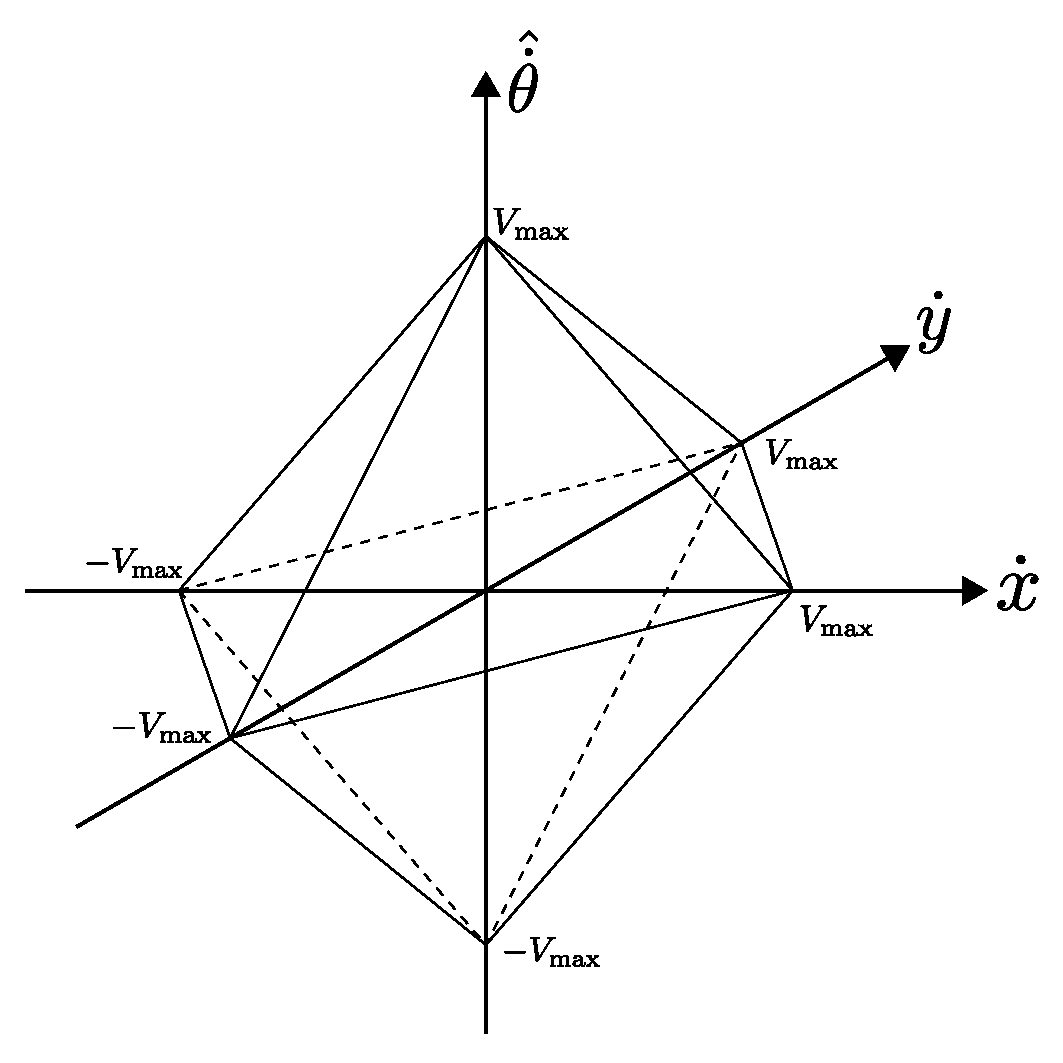
\includegraphics[width=80truemm, clip]{images/constraint.pdf}
    \caption{Constraint Area of Input Velocity Vector}
    \label{fig:constraint}
  \end{figure}

  \subsection{入力信号から速度ベクトルへのマッピング}

  \subsubsection{コントローラからの入力信号}

  ここでは3軸のアナログジョイスティックを用いてロボットを速度制御することを考える.
  それぞれのアナログジョイスティックの入力は$\dot{x}$,$\dot{y}$,$\hat{\dot{\theta}}$に対応するものとし,$\dot{x}$に対応するアナログジョイスティックの信号値を$\alpha$,$\dot{y}$に対応するものを$\beta$,$\hat{\dot{\theta}}$に対応するものを$\gamma$と表す.
  また,各ジョイスティックの信号値の範囲は-1.0~1.0であるとする.

  3つのジョイスティックによる入力の組み合わせをベクトル$\vec{\epsilon} = (\alpha, \beta, \gamma)^T$で表す.
  $\alpha\beta\gamma$座標系において,$\vec{\epsilon}$が取る領域は,原点を中心とする幅2の立方体となる.
  この立方体の領域を,図\ref{fig:constraint}に示す正八面体にマッピングすることで,ジョイスティックによる制御が可能になる.

  \begin{figure}[h]
    \centering
    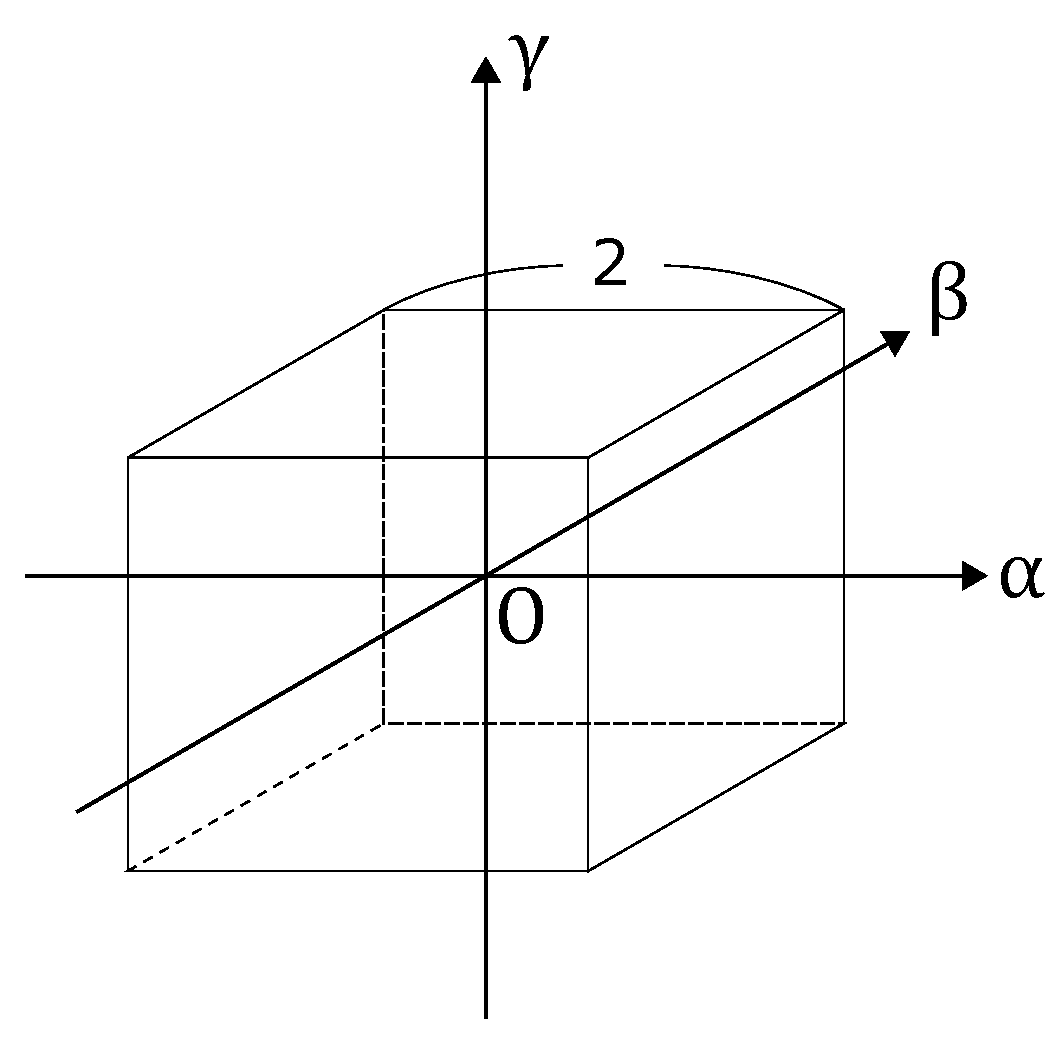
\includegraphics[width=80truemm, clip]{images/input.pdf}
    \caption{Input Area}
    \label{fig:input}
  \end{figure}

  \subsubsection{極座標変換によるアプローチ}

  立方体領域から正八面体領域へのマッピングを直接行うのは困難であるため,ここでは極座標変換を用いたマッピング処理を行う.

  最初の段階として,$\alpha\beta\gamma$座標系における立方体領域を3次元極座標における球面へ変換する.
  まず入力信号ベクトル$\vec{\epsilon}$を図\ref{fig:signal_vector}に示すように極座標表示し,ベクトルの向き$(\phi, \xi)$と信号強度$\sigma$を求める.

  \begin{figure}[ht]
    \centering
    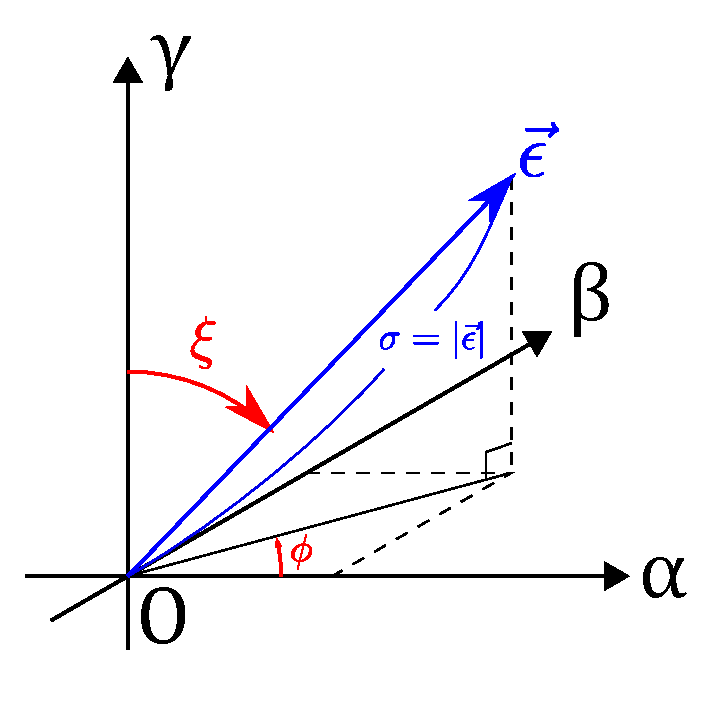
\includegraphics[width=60truemm, clip]{images/signal_vector.pdf}
    \caption{Input Signal Vector with Polar Coordinates}
    \label{fig:signal_vector}
  \end{figure}

  向き$(\phi, \xi)$はそれぞれ$\phi = \arccos{\frac{\alpha}{\sqrt{\alpha^2 + \beta^2}}}$,$\xi = \arccos{\frac{\gamma}{\sqrt{\alpha^2 + \beta^2 + \gamma^2}}}$である.
  また,$\vec{\epsilon}$の大きさは$|\vec{\epsilon}| = \sqrt{\alpha^2 + \beta^2 + \gamma^2}$から求められるが,$\alpha$,$\beta$,$\gamma$の値によっては$\vec{\epsilon}$の大きさは1.0を超えてしまう.
  これを防ぐために正規化処理を行う.
  $\vec{\epsilon}$は立方体領域内部に存在するので,$\vec{\epsilon}$の大きさの取りうる最大値は$\vec{\epsilon}$の向きによって決定される.
  $\vec{\epsilon}$が取りうる最大値で$\vec{\epsilon}$の大きさを除することで,$\vec{\epsilon}$の大きさを正規化し,信号の強度$\sigma$を求めることができる.

  まずは向き$(\phi, \xi)$で取りうる$|\vec{\epsilon}|$の最大値$\sigma_{\text{max}}$を求める.
  $\vec{\epsilon}$が立方体のどの面に属するかは,向き$(\phi, \xi)$によって決まる.
  $\phi$の範囲区分は4つあり,$\phi$の値によって立方体のどの側面が候補になるかが決まる.
  また,$\xi$の範囲によって$\vec{\epsilon}$が立方体の底面に属するかどうかが定まる.
  図\ref{fig:range_of_xi}に示す通り,$\xi$の閾値$\xi_{\text{th}}$は$\phi$の値に依存する.
  $\xi_{\text{th}} \leq \xi \leq (\pi - \xi_{\text{th}})$のとき$\vec{\epsilon}$は立方体の側面に属し,
  それ以外のときは立方体の底面に属する.
  図\ref{fig:range_of_xi}より,$\xi_{\text{th}} = \arctan{\frac{1}{\cos{\phi}}}$である.

  \begin{figure}[ht]
    \centering
    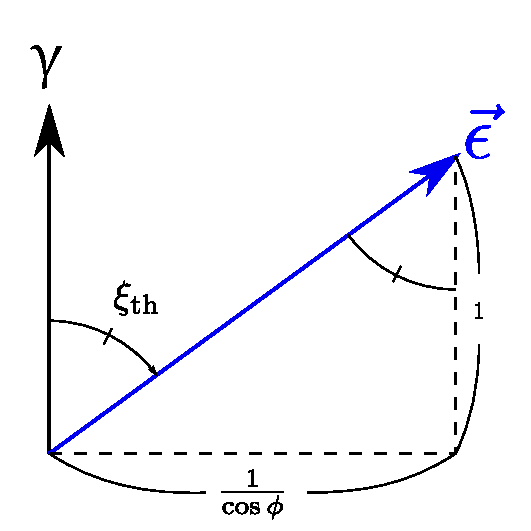
\includegraphics[width=60truemm, clip]{images/range_of_xi.pdf}
    \label{fig:range_of_xi}
    \caption{Range of \xi}
  \end{figure}

  以上を踏まえて立方体の式を極座標で表すと,

  \begin{subequations}
    \begin{empheq}[left=\empheqlbrace]{alignat=2}
      \alpha = 1 & \quad (0 \leq \phi \leq \frac{\pi}{4}, \frac{7\pi}{4} \leq \phi \leq 2\pi, \xi_{\text{th}} \leq \xi \leq (\pi - \xi_{\text{th}})) \\
      \beta = 1 & \quad (\frac{\pi}{4} \leq \phi < \frac{3\pi}{4}, \xi_{\text{th}} \leq \xi \leq (\pi - \xi_{\text{th}})) \\
      \gamma = 1 & \quad (\xi < \xi_{\text{th}}) \\
      \alpha = -1 & \quad (\frac{3\pi}{4} \leq \phi < \frac{5\pi}{4}, \xi_{\text{th}} \leq \xi \leq (\pi - \xi_{\text{th}})) \\
      \beta = -1 & \quad (\frac{5\pi}{4} \leq \phi < \frac{7\pi}{4}, \xi_{\text{th}} \leq \xi \leq (\pi - \xi_{\text{th}})) \\
      \gamma = -1 & \quad (\xi > (\pi - \xi_{\text{th}}))
    \end{empheq}
    \label{eq:polarized_cube}
  \end{subequations}

\end{document}